\documentclass[11pt,a4paper]{article}

\usepackage[a4paper,margin=2.2cm]{geometry}
\usepackage[italian]{babel}
\usepackage{lmodern}
\usepackage{microtype}
\usepackage{booktabs}
\usepackage{tabularx}
\usepackage{multirow}
\usepackage{makecell}
\usepackage{graphicx}
\usepackage{float}
\usepackage[font=small,labelfont=bf]{caption}
\usepackage{enumitem}
\usepackage{xcolor}
\usepackage{listings}
\usepackage[hidelinks]{hyperref}

\setlist{itemsep=1pt,topsep=3pt}
\setlength{\parskip}{3pt}
\setlength{\emergencystretch}{3em}

\definecolor{codebg}{RGB}{246,247,249}
\definecolor{codekw}{RGB}{0,82,147}
\definecolor{codecm}{RGB}{110,110,110}
\lstset{basicstyle=\ttfamily\scriptsize, backgroundcolor=\color{codebg}, frame=single, rulecolor=\color{gray!40},
  keywordstyle=\color{codekw}\bfseries, commentstyle=\color{codecm}\itshape, columns=fullflexible,
  keepspaces=true, breaklines=true, aboveskip=4pt, belowskip=4pt,
  literate={à}{{\`a}}1 {è}{{\`e}}1 {ì}{{\`i}}1 {ò}{{\`o}}1 {ù}{{\`u}}1 {←}{{$\leftarrow$}}1 {→}{{$\rightarrow$}}1 {∪}{{$\cup$}}1}
\lstdefinelanguage{pseudo}{morekeywords={per,ogni,se,in}, sensitive=true, morecomment=[l]{//}}

% --- Numeri misurati, generati da genera_dati.py -----------------------------------------------
\expandafter\def\csname t:local:hive:job_1:flights_1\endcsname{12,3}
\expandafter\def\csname e:local:hive:job_1:flights_1\endcsname{6,5}
\expandafter\def\csname o:local:hive:job_1:flights_1\endcsname{5,9}
\expandafter\def\csname t:local:hive:job_1:flights_20\endcsname{13,8}
\expandafter\def\csname e:local:hive:job_1:flights_20\endcsname{7,5}
\expandafter\def\csname o:local:hive:job_1:flights_20\endcsname{6,3}
\expandafter\def\csname t:local:hive:job_1:flights_50\endcsname{16,8}
\expandafter\def\csname e:local:hive:job_1:flights_50\endcsname{10,6}
\expandafter\def\csname o:local:hive:job_1:flights_50\endcsname{6,2}
\expandafter\def\csname t:local:hive:job_1:flights_70\endcsname{18,0}
\expandafter\def\csname e:local:hive:job_1:flights_70\endcsname{11,5}
\expandafter\def\csname o:local:hive:job_1:flights_70\endcsname{6,5}
\expandafter\def\csname t:local:hive:job_1:flights_cleaned\endcsname{21,3}
\expandafter\def\csname e:local:hive:job_1:flights_cleaned\endcsname{14,7}
\expandafter\def\csname o:local:hive:job_1:flights_cleaned\endcsname{6,6}
\expandafter\def\csname t:local:hive:job_1:flights_x2\endcsname{43,0}
\expandafter\def\csname e:local:hive:job_1:flights_x2\endcsname{34,0}
\expandafter\def\csname o:local:hive:job_1:flights_x2\endcsname{9,0}
\expandafter\def\csname t:local:hive:job_1:flights_x5\endcsname{59,8}
\expandafter\def\csname e:local:hive:job_1:flights_x5\endcsname{52,5}
\expandafter\def\csname o:local:hive:job_1:flights_x5\endcsname{7,3}
\expandafter\def\csname t:local:hive:job_2:flights_1\endcsname{21,8}
\expandafter\def\csname e:local:hive:job_2:flights_1\endcsname{15,5}
\expandafter\def\csname o:local:hive:job_2:flights_1\endcsname{6,3}
\expandafter\def\csname t:local:hive:job_2:flights_20\endcsname{23,4}
\expandafter\def\csname e:local:hive:job_2:flights_20\endcsname{16,9}
\expandafter\def\csname o:local:hive:job_2:flights_20\endcsname{6,5}
\expandafter\def\csname t:local:hive:job_2:flights_50\endcsname{26,6}
\expandafter\def\csname e:local:hive:job_2:flights_50\endcsname{20,0}
\expandafter\def\csname o:local:hive:job_2:flights_50\endcsname{6,6}
\expandafter\def\csname t:local:hive:job_2:flights_70\endcsname{29,2}
\expandafter\def\csname e:local:hive:job_2:flights_70\endcsname{22,4}
\expandafter\def\csname o:local:hive:job_2:flights_70\endcsname{6,8}
\expandafter\def\csname t:local:hive:job_2:flights_cleaned\endcsname{34,4}
\expandafter\def\csname e:local:hive:job_2:flights_cleaned\endcsname{27,2}
\expandafter\def\csname o:local:hive:job_2:flights_cleaned\endcsname{7,2}
\expandafter\def\csname t:local:hive:job_2:flights_x2\endcsname{46,5}
\expandafter\def\csname e:local:hive:job_2:flights_x2\endcsname{38,8}
\expandafter\def\csname o:local:hive:job_2:flights_x2\endcsname{7,6}
\expandafter\def\csname t:local:hive:job_2:flights_x5\endcsname{82,4}
\expandafter\def\csname e:local:hive:job_2:flights_x5\endcsname{74,5}
\expandafter\def\csname o:local:hive:job_2:flights_x5\endcsname{7,8}
\expandafter\def\csname t:local:spark-core:job_1:flights_1\endcsname{6,7}
\expandafter\def\csname e:local:spark-core:job_1:flights_1\endcsname{3,5}
\expandafter\def\csname o:local:spark-core:job_1:flights_1\endcsname{3,3}
\expandafter\def\csname t:local:spark-core:job_1:flights_20\endcsname{8,0}
\expandafter\def\csname e:local:spark-core:job_1:flights_20\endcsname{4,9}
\expandafter\def\csname o:local:spark-core:job_1:flights_20\endcsname{3,1}
\expandafter\def\csname t:local:spark-core:job_1:flights_50\endcsname{10,9}
\expandafter\def\csname e:local:spark-core:job_1:flights_50\endcsname{7,8}
\expandafter\def\csname o:local:spark-core:job_1:flights_50\endcsname{3,1}
\expandafter\def\csname t:local:spark-core:job_1:flights_70\endcsname{13,2}
\expandafter\def\csname e:local:spark-core:job_1:flights_70\endcsname{10,1}
\expandafter\def\csname o:local:spark-core:job_1:flights_70\endcsname{3,1}
\expandafter\def\csname t:local:spark-core:job_1:flights_cleaned\endcsname{16,6}
\expandafter\def\csname e:local:spark-core:job_1:flights_cleaned\endcsname{13,3}
\expandafter\def\csname o:local:spark-core:job_1:flights_cleaned\endcsname{3,3}
\expandafter\def\csname t:local:spark-core:job_1:flights_x2\endcsname{22,7}
\expandafter\def\csname e:local:spark-core:job_1:flights_x2\endcsname{19,2}
\expandafter\def\csname o:local:spark-core:job_1:flights_x2\endcsname{3,5}
\expandafter\def\csname t:local:spark-core:job_1:flights_x5\endcsname{43,5}
\expandafter\def\csname e:local:spark-core:job_1:flights_x5\endcsname{40,0}
\expandafter\def\csname o:local:spark-core:job_1:flights_x5\endcsname{3,5}
\expandafter\def\csname t:local:spark-core:job_2:flights_1\endcsname{7,1}
\expandafter\def\csname e:local:spark-core:job_2:flights_1\endcsname{4,0}
\expandafter\def\csname o:local:spark-core:job_2:flights_1\endcsname{3,1}
\expandafter\def\csname t:local:spark-core:job_2:flights_20\endcsname{9,6}
\expandafter\def\csname e:local:spark-core:job_2:flights_20\endcsname{6,5}
\expandafter\def\csname o:local:spark-core:job_2:flights_20\endcsname{3,1}
\expandafter\def\csname t:local:spark-core:job_2:flights_50\endcsname{14,3}
\expandafter\def\csname e:local:spark-core:job_2:flights_50\endcsname{11,2}
\expandafter\def\csname o:local:spark-core:job_2:flights_50\endcsname{3,1}
\expandafter\def\csname t:local:spark-core:job_2:flights_70\endcsname{19,7}
\expandafter\def\csname e:local:spark-core:job_2:flights_70\endcsname{16,1}
\expandafter\def\csname o:local:spark-core:job_2:flights_70\endcsname{3,6}
\expandafter\def\csname t:local:spark-core:job_2:flights_cleaned\endcsname{24,6}
\expandafter\def\csname e:local:spark-core:job_2:flights_cleaned\endcsname{21,3}
\expandafter\def\csname o:local:spark-core:job_2:flights_cleaned\endcsname{3,4}
\expandafter\def\csname t:local:spark-core:job_2:flights_x2\endcsname{46,1}
\expandafter\def\csname e:local:spark-core:job_2:flights_x2\endcsname{42,0}
\expandafter\def\csname o:local:spark-core:job_2:flights_x2\endcsname{4,0}
\expandafter\def\csname t:local:spark-core:job_2:flights_x5\endcsname{77,0}
\expandafter\def\csname e:local:spark-core:job_2:flights_x5\endcsname{73,6}
\expandafter\def\csname o:local:spark-core:job_2:flights_x5\endcsname{3,4}
\expandafter\def\csname t:local:spark-sql:job_1:flights_1\endcsname{7,1}
\expandafter\def\csname e:local:spark-sql:job_1:flights_1\endcsname{4,7}
\expandafter\def\csname o:local:spark-sql:job_1:flights_1\endcsname{2,5}
\expandafter\def\csname t:local:spark-sql:job_1:flights_20\endcsname{9,2}
\expandafter\def\csname e:local:spark-sql:job_1:flights_20\endcsname{7,0}
\expandafter\def\csname o:local:spark-sql:job_1:flights_20\endcsname{2,2}
\expandafter\def\csname t:local:spark-sql:job_1:flights_50\endcsname{13,2}
\expandafter\def\csname e:local:spark-sql:job_1:flights_50\endcsname{10,6}
\expandafter\def\csname o:local:spark-sql:job_1:flights_50\endcsname{2,5}
\expandafter\def\csname t:local:spark-sql:job_1:flights_70\endcsname{13,7}
\expandafter\def\csname e:local:spark-sql:job_1:flights_70\endcsname{11,3}
\expandafter\def\csname o:local:spark-sql:job_1:flights_70\endcsname{2,4}
\expandafter\def\csname t:local:spark-sql:job_1:flights_cleaned\endcsname{17,5}
\expandafter\def\csname e:local:spark-sql:job_1:flights_cleaned\endcsname{15,0}
\expandafter\def\csname o:local:spark-sql:job_1:flights_cleaned\endcsname{2,4}
\expandafter\def\csname t:local:spark-sql:job_1:flights_x2\endcsname{32,9}
\expandafter\def\csname e:local:spark-sql:job_1:flights_x2\endcsname{30,1}
\expandafter\def\csname o:local:spark-sql:job_1:flights_x2\endcsname{2,8}
\expandafter\def\csname t:local:spark-sql:job_1:flights_x5\endcsname{70,2}
\expandafter\def\csname e:local:spark-sql:job_1:flights_x5\endcsname{67,5}
\expandafter\def\csname o:local:spark-sql:job_1:flights_x5\endcsname{2,7}
\expandafter\def\csname t:local:spark-sql:job_2:flights_1\endcsname{7,6}
\expandafter\def\csname e:local:spark-sql:job_2:flights_1\endcsname{5,2}
\expandafter\def\csname o:local:spark-sql:job_2:flights_1\endcsname{2,4}
\expandafter\def\csname t:local:spark-sql:job_2:flights_20\endcsname{10,7}
\expandafter\def\csname e:local:spark-sql:job_2:flights_20\endcsname{8,3}
\expandafter\def\csname o:local:spark-sql:job_2:flights_20\endcsname{2,3}
\expandafter\def\csname t:local:spark-sql:job_2:flights_50\endcsname{13,2}
\expandafter\def\csname e:local:spark-sql:job_2:flights_50\endcsname{10,8}
\expandafter\def\csname o:local:spark-sql:job_2:flights_50\endcsname{2,4}
\expandafter\def\csname t:local:spark-sql:job_2:flights_70\endcsname{16,6}
\expandafter\def\csname e:local:spark-sql:job_2:flights_70\endcsname{13,7}
\expandafter\def\csname o:local:spark-sql:job_2:flights_70\endcsname{2,9}
\expandafter\def\csname t:local:spark-sql:job_2:flights_cleaned\endcsname{20,7}
\expandafter\def\csname e:local:spark-sql:job_2:flights_cleaned\endcsname{18,1}
\expandafter\def\csname o:local:spark-sql:job_2:flights_cleaned\endcsname{2,6}
\expandafter\def\csname t:local:spark-sql:job_2:flights_x2\endcsname{37,9}
\expandafter\def\csname e:local:spark-sql:job_2:flights_x2\endcsname{34,4}
\expandafter\def\csname o:local:spark-sql:job_2:flights_x2\endcsname{3,4}
\expandafter\def\csname t:local:spark-sql:job_2:flights_x5\endcsname{73,9}
\expandafter\def\csname e:local:spark-sql:job_2:flights_x5\endcsname{71,2}
\expandafter\def\csname o:local:spark-sql:job_2:flights_x5\endcsname{2,7}
\expandafter\def\csname t:yarn:hive:job_1:flights_1\endcsname{49,3}
\expandafter\def\csname e:yarn:hive:job_1:flights_1\endcsname{42,7}
\expandafter\def\csname o:yarn:hive:job_1:flights_1\endcsname{6,7}
\expandafter\def\csname t:yarn:hive:job_1:flights_20\endcsname{46,9}
\expandafter\def\csname e:yarn:hive:job_1:flights_20\endcsname{40,5}
\expandafter\def\csname o:yarn:hive:job_1:flights_20\endcsname{6,4}
\expandafter\def\csname t:yarn:hive:job_1:flights_50\endcsname{50,1}
\expandafter\def\csname e:yarn:hive:job_1:flights_50\endcsname{44,0}
\expandafter\def\csname o:yarn:hive:job_1:flights_50\endcsname{6,2}
\expandafter\def\csname t:yarn:hive:job_1:flights_70\endcsname{51,1}
\expandafter\def\csname e:yarn:hive:job_1:flights_70\endcsname{45,2}
\expandafter\def\csname o:yarn:hive:job_1:flights_70\endcsname{6,0}
\expandafter\def\csname t:yarn:hive:job_1:flights_cleaned\endcsname{51,4}
\expandafter\def\csname e:yarn:hive:job_1:flights_cleaned\endcsname{45,5}
\expandafter\def\csname o:yarn:hive:job_1:flights_cleaned\endcsname{5,9}
\expandafter\def\csname t:yarn:hive:job_1:flights_x2\endcsname{59,2}
\expandafter\def\csname e:yarn:hive:job_1:flights_x2\endcsname{52,4}
\expandafter\def\csname o:yarn:hive:job_1:flights_x2\endcsname{6,8}
\expandafter\def\csname t:yarn:hive:job_1:flights_x5\endcsname{71,9}
\expandafter\def\csname e:yarn:hive:job_1:flights_x5\endcsname{65,2}
\expandafter\def\csname o:yarn:hive:job_1:flights_x5\endcsname{6,7}
\expandafter\def\csname t:yarn:hive:job_2:flights_1\endcsname{146,0}
\expandafter\def\csname e:yarn:hive:job_2:flights_1\endcsname{138,2}
\expandafter\def\csname o:yarn:hive:job_2:flights_1\endcsname{7,8}
\expandafter\def\csname t:yarn:hive:job_2:flights_20\endcsname{130,6}
\expandafter\def\csname e:yarn:hive:job_2:flights_20\endcsname{123,8}
\expandafter\def\csname o:yarn:hive:job_2:flights_20\endcsname{6,8}
\expandafter\def\csname t:yarn:hive:job_2:flights_50\endcsname{137,7}
\expandafter\def\csname e:yarn:hive:job_2:flights_50\endcsname{130,0}
\expandafter\def\csname o:yarn:hive:job_2:flights_50\endcsname{7,7}
\expandafter\def\csname t:yarn:hive:job_2:flights_70\endcsname{135,2}
\expandafter\def\csname e:yarn:hive:job_2:flights_70\endcsname{128,7}
\expandafter\def\csname o:yarn:hive:job_2:flights_70\endcsname{6,5}
\expandafter\def\csname t:yarn:hive:job_2:flights_cleaned\endcsname{158,9}
\expandafter\def\csname e:yarn:hive:job_2:flights_cleaned\endcsname{151,3}
\expandafter\def\csname o:yarn:hive:job_2:flights_cleaned\endcsname{7,6}
\expandafter\def\csname t:yarn:hive:job_2:flights_x2\endcsname{144,0}
\expandafter\def\csname e:yarn:hive:job_2:flights_x2\endcsname{136,5}
\expandafter\def\csname o:yarn:hive:job_2:flights_x2\endcsname{7,6}
\expandafter\def\csname t:yarn:hive:job_2:flights_x5\endcsname{184,2}
\expandafter\def\csname e:yarn:hive:job_2:flights_x5\endcsname{175,7}
\expandafter\def\csname o:yarn:hive:job_2:flights_x5\endcsname{8,5}
\expandafter\def\csname t:yarn:spark-core:job_1:flights_1\endcsname{20,1}
\expandafter\def\csname e:yarn:spark-core:job_1:flights_1\endcsname{16,7}
\expandafter\def\csname o:yarn:spark-core:job_1:flights_1\endcsname{3,4}
\expandafter\def\csname t:yarn:spark-core:job_1:flights_20\endcsname{21,6}
\expandafter\def\csname e:yarn:spark-core:job_1:flights_20\endcsname{18,4}
\expandafter\def\csname o:yarn:spark-core:job_1:flights_20\endcsname{3,2}
\expandafter\def\csname t:yarn:spark-core:job_1:flights_50\endcsname{22,6}
\expandafter\def\csname e:yarn:spark-core:job_1:flights_50\endcsname{19,5}
\expandafter\def\csname o:yarn:spark-core:job_1:flights_50\endcsname{3,1}
\expandafter\def\csname t:yarn:spark-core:job_1:flights_70\endcsname{27,7}
\expandafter\def\csname e:yarn:spark-core:job_1:flights_70\endcsname{24,1}
\expandafter\def\csname o:yarn:spark-core:job_1:flights_70\endcsname{3,6}
\expandafter\def\csname t:yarn:spark-core:job_1:flights_cleaned\endcsname{26,4}
\expandafter\def\csname e:yarn:spark-core:job_1:flights_cleaned\endcsname{23,3}
\expandafter\def\csname o:yarn:spark-core:job_1:flights_cleaned\endcsname{3,1}
\expandafter\def\csname t:yarn:spark-core:job_1:flights_x2\endcsname{36,3}
\expandafter\def\csname e:yarn:spark-core:job_1:flights_x2\endcsname{33,1}
\expandafter\def\csname o:yarn:spark-core:job_1:flights_x2\endcsname{3,1}
\expandafter\def\csname t:yarn:spark-core:job_1:flights_x5\endcsname{63,2}
\expandafter\def\csname e:yarn:spark-core:job_1:flights_x5\endcsname{60,0}
\expandafter\def\csname o:yarn:spark-core:job_1:flights_x5\endcsname{3,2}
\expandafter\def\csname t:yarn:spark-core:job_2:flights_1\endcsname{18,9}
\expandafter\def\csname e:yarn:spark-core:job_2:flights_1\endcsname{15,7}
\expandafter\def\csname o:yarn:spark-core:job_2:flights_1\endcsname{3,1}
\expandafter\def\csname t:yarn:spark-core:job_2:flights_20\endcsname{23,0}
\expandafter\def\csname e:yarn:spark-core:job_2:flights_20\endcsname{19,8}
\expandafter\def\csname o:yarn:spark-core:job_2:flights_20\endcsname{3,2}
\expandafter\def\csname t:yarn:spark-core:job_2:flights_50\endcsname{27,2}
\expandafter\def\csname e:yarn:spark-core:job_2:flights_50\endcsname{24,1}
\expandafter\def\csname o:yarn:spark-core:job_2:flights_50\endcsname{3,1}
\expandafter\def\csname t:yarn:spark-core:job_2:flights_70\endcsname{29,7}
\expandafter\def\csname e:yarn:spark-core:job_2:flights_70\endcsname{26,6}
\expandafter\def\csname o:yarn:spark-core:job_2:flights_70\endcsname{3,2}
\expandafter\def\csname t:yarn:spark-core:job_2:flights_cleaned\endcsname{33,6}
\expandafter\def\csname e:yarn:spark-core:job_2:flights_cleaned\endcsname{30,5}
\expandafter\def\csname o:yarn:spark-core:job_2:flights_cleaned\endcsname{3,1}
\expandafter\def\csname t:yarn:spark-core:job_2:flights_x2\endcsname{56,0}
\expandafter\def\csname e:yarn:spark-core:job_2:flights_x2\endcsname{52,9}
\expandafter\def\csname o:yarn:spark-core:job_2:flights_x2\endcsname{3,1}
\expandafter\def\csname t:yarn:spark-core:job_2:flights_x5\endcsname{113,5}
\expandafter\def\csname e:yarn:spark-core:job_2:flights_x5\endcsname{110,3}
\expandafter\def\csname o:yarn:spark-core:job_2:flights_x5\endcsname{3,2}
\expandafter\def\csname t:yarn:spark-sql:job_1:flights_1\endcsname{20,9}
\expandafter\def\csname e:yarn:spark-sql:job_1:flights_1\endcsname{18,7}
\expandafter\def\csname o:yarn:spark-sql:job_1:flights_1\endcsname{2,3}
\expandafter\def\csname t:yarn:spark-sql:job_1:flights_20\endcsname{25,5}
\expandafter\def\csname e:yarn:spark-sql:job_1:flights_20\endcsname{23,3}
\expandafter\def\csname o:yarn:spark-sql:job_1:flights_20\endcsname{2,3}
\expandafter\def\csname t:yarn:spark-sql:job_1:flights_50\endcsname{29,6}
\expandafter\def\csname e:yarn:spark-sql:job_1:flights_50\endcsname{27,0}
\expandafter\def\csname o:yarn:spark-sql:job_1:flights_50\endcsname{2,6}
\expandafter\def\csname t:yarn:spark-sql:job_1:flights_70\endcsname{32,3}
\expandafter\def\csname e:yarn:spark-sql:job_1:flights_70\endcsname{29,7}
\expandafter\def\csname o:yarn:spark-sql:job_1:flights_70\endcsname{2,6}
\expandafter\def\csname t:yarn:spark-sql:job_1:flights_cleaned\endcsname{34,9}
\expandafter\def\csname e:yarn:spark-sql:job_1:flights_cleaned\endcsname{32,4}
\expandafter\def\csname o:yarn:spark-sql:job_1:flights_cleaned\endcsname{2,4}
\expandafter\def\csname t:yarn:spark-sql:job_1:flights_x2\endcsname{58,6}
\expandafter\def\csname e:yarn:spark-sql:job_1:flights_x2\endcsname{55,9}
\expandafter\def\csname o:yarn:spark-sql:job_1:flights_x2\endcsname{2,7}
\expandafter\def\csname t:yarn:spark-sql:job_1:flights_x5\endcsname{110,8}
\expandafter\def\csname e:yarn:spark-sql:job_1:flights_x5\endcsname{108,5}
\expandafter\def\csname o:yarn:spark-sql:job_1:flights_x5\endcsname{2,3}
\expandafter\def\csname t:yarn:spark-sql:job_2:flights_1\endcsname{24,0}
\expandafter\def\csname e:yarn:spark-sql:job_2:flights_1\endcsname{21,4}
\expandafter\def\csname o:yarn:spark-sql:job_2:flights_1\endcsname{2,6}
\expandafter\def\csname t:yarn:spark-sql:job_2:flights_20\endcsname{26,0}
\expandafter\def\csname e:yarn:spark-sql:job_2:flights_20\endcsname{23,6}
\expandafter\def\csname o:yarn:spark-sql:job_2:flights_20\endcsname{2,4}
\expandafter\def\csname t:yarn:spark-sql:job_2:flights_50\endcsname{28,6}
\expandafter\def\csname e:yarn:spark-sql:job_2:flights_50\endcsname{26,4}
\expandafter\def\csname o:yarn:spark-sql:job_2:flights_50\endcsname{2,1}
\expandafter\def\csname t:yarn:spark-sql:job_2:flights_70\endcsname{35,6}
\expandafter\def\csname e:yarn:spark-sql:job_2:flights_70\endcsname{33,0}
\expandafter\def\csname o:yarn:spark-sql:job_2:flights_70\endcsname{2,6}
\expandafter\def\csname t:yarn:spark-sql:job_2:flights_cleaned\endcsname{43,6}
\expandafter\def\csname e:yarn:spark-sql:job_2:flights_cleaned\endcsname{40,8}
\expandafter\def\csname o:yarn:spark-sql:job_2:flights_cleaned\endcsname{2,8}
\expandafter\def\csname t:yarn:spark-sql:job_2:flights_x2\endcsname{61,8}
\expandafter\def\csname e:yarn:spark-sql:job_2:flights_x2\endcsname{59,4}
\expandafter\def\csname o:yarn:spark-sql:job_2:flights_x2\endcsname{2,4}
\expandafter\def\csname t:yarn:spark-sql:job_2:flights_x5\endcsname{141,7}
\expandafter\def\csname e:yarn:spark-sql:job_2:flights_x5\endcsname{138,7}
\expandafter\def\csname o:yarn:spark-sql:job_2:flights_x5\endcsname{3,0}
\expandafter\def\csname t:aws:spark-core:job_1:flights_1\endcsname{31,9}
\expandafter\def\csname t:aws:spark-core:job_1:flights_20\endcsname{35,3}
\expandafter\def\csname t:aws:spark-core:job_1:flights_50\endcsname{39,1}
\expandafter\def\csname t:aws:spark-core:job_1:flights_70\endcsname{46,8}
\expandafter\def\csname t:aws:spark-core:job_1:flights_cleaned\endcsname{48,3}
\expandafter\def\csname t:aws:spark-sql:job_1:flights_1\endcsname{36,4}
\expandafter\def\csname t:aws:spark-sql:job_1:flights_20\endcsname{41,9}
\expandafter\def\csname t:aws:spark-sql:job_1:flights_50\endcsname{48,7}
\expandafter\def\csname t:aws:spark-sql:job_1:flights_70\endcsname{48,0}
\expandafter\def\csname t:aws:spark-sql:job_1:flights_cleaned\endcsname{52,4}
\expandafter\def\csname t:aws:hive:job_1:flights_1\endcsname{35,8}
\expandafter\def\csname t:aws:hive:job_1:flights_20\endcsname{32,7}
\expandafter\def\csname t:aws:hive:job_1:flights_50\endcsname{40,2}
\expandafter\def\csname t:aws:hive:job_1:flights_70\endcsname{40,6}
\expandafter\def\csname t:aws:hive:job_1:flights_cleaned\endcsname{43,1}
\expandafter\def\csname t:aws:spark-core:job_2:flights_1\endcsname{28,0}
\expandafter\def\csname t:aws:spark-core:job_2:flights_20\endcsname{36,4}
\expandafter\def\csname t:aws:spark-core:job_2:flights_50\endcsname{41,1}
\expandafter\def\csname t:aws:spark-core:job_2:flights_70\endcsname{49,7}
\expandafter\def\csname t:aws:spark-core:job_2:flights_cleaned\endcsname{50,8}
\expandafter\def\csname t:aws:spark-sql:job_2:flights_1\endcsname{37,9}
\expandafter\def\csname t:aws:spark-sql:job_2:flights_20\endcsname{44,9}
\expandafter\def\csname t:aws:spark-sql:job_2:flights_50\endcsname{50,5}
\expandafter\def\csname t:aws:spark-sql:job_2:flights_70\endcsname{53,0}
\expandafter\def\csname t:aws:spark-sql:job_2:flights_cleaned\endcsname{59,1}
\expandafter\def\csname t:aws:hive:job_2:flights_1\endcsname{38,4}
\expandafter\def\csname t:aws:hive:job_2:flights_20\endcsname{42,6}
\expandafter\def\csname t:aws:hive:job_2:flights_50\endcsname{42,7}
\expandafter\def\csname t:aws:hive:job_2:flights_70\endcsname{48,5}
\expandafter\def\csname t:aws:hive:job_2:flights_cleaned\endcsname{54,0}
\expandafter\def\csname q:righe_iniziali\endcsname{7.079.081}
\expandafter\def\csname q:righe_finali\endcsname{7.061.582}
\expandafter\def\csname q:colonne_iniziali\endcsname{35}
\expandafter\def\csname q:dirottato\endcsname{17.499}
\expandafter\def\csname q:campi_chiave_mancanti\endcsname{0}
\expandafter\def\csname q:mese_non_valido\endcsname{0}
\expandafter\def\csname q:codice_aeroporto_non_valido\endcsname{0}
\expandafter\def\csname q:cancellazione_incoerente\endcsname{0}
\expandafter\def\csname q:ritardi_mancanti\endcsname{0}
\expandafter\def\csname q:cause_incoerenti\endcsname{0}
\expandafter\def\csname q:duplicati\endcsname{0}
\expandafter\def\csname q:ritardo_cancellati\endcsname{3.345}
\expandafter\def\csname q:causa_prevalente\endcsname{1.449.970}
\expandafter\def\csname q:escluse\endcsname{17.499}
\expandafter\def\csname q:escluse_pct\endcsname{0,25}
\expandafter\def\csname q:cancellati\endcsname{96.315}
\expandafter\def\csname q:ritardo_partenza_oltre_24h\endcsname{556}
\expandafter\def\csname q:ritardo_arrivo_oltre_24h\endcsname{567}
\expandafter\def\csname q:dep_delay_min\endcsname{-96}
\expandafter\def\csname q:dep_delay_max\endcsname{3.777}
\expandafter\def\csname q:arr_delay_min\endcsname{-126}
\expandafter\def\csname q:arr_delay_max\endcsname{3.803}
\expandafter\def\csname q:compagnie\endcsname{15}
\expandafter\def\csname q:aeroporti_partenza\endcsname{348}
\expandafter\def\csname q:aeroporti_sotto_soglia\endcsname{3}
\expandafter\def\csname q:voli_aeroporti_sotto_soglia\endcsname{99}
\expandafter\def\csname q:soglia_aeroporti_voli\endcsname{50}
\expandafter\def\csname q:null_month\endcsname{0}
\expandafter\def\csname q:null_op_unique_carrier\endcsname{0}
\expandafter\def\csname q:null_origin\endcsname{0}
\expandafter\def\csname q:null_dest\endcsname{0}
\expandafter\def\csname q:null_dep_delay\endcsname{96.315}
\expandafter\def\csname q:null_arr_delay\endcsname{96.315}
\expandafter\def\csname q:null_cancelled\endcsname{0}
\expandafter\def\csname q:null_cancellation_code\endcsname{6.965.267}
\expandafter\def\csname q:null_delay_code\endcsname{5.611.612}
\expandafter\def\csname ds:righe:flights_1\endcsname{71.085}
\expandafter\def\csname ds:mb:flights_1\endcsname{2,1}
\expandafter\def\csname ds:righe:flights_20\endcsname{1.413.555}
\expandafter\def\csname ds:mb:flights_20\endcsname{41,1}
\expandafter\def\csname ds:righe:flights_50\endcsname{3.531.974}
\expandafter\def\csname ds:mb:flights_50\endcsname{102,8}
\expandafter\def\csname ds:righe:flights_70\endcsname{4.943.811}
\expandafter\def\csname ds:mb:flights_70\endcsname{143,8}
\expandafter\def\csname ds:righe:flights_cleaned\endcsname{7.061.582}
\expandafter\def\csname ds:mb:flights_cleaned\endcsname{205,5}
\expandafter\def\csname ds:righe:flights_x2\endcsname{14.123.164}
\expandafter\def\csname ds:mb:flights_x2\endcsname{410,9}
\expandafter\def\csname ds:righe:flights_x5\endcsname{35.307.910}
\expandafter\def\csname ds:mb:flights_x5\endcsname{1.027,3}
\expandafter\def\csname r:yarn:spark-core:job_1\endcsname{1,58}
\expandafter\def\csname r:aws:spark-core:job_1\endcsname{2,90}
\expandafter\def\csname r:yarn:spark-sql:job_1\endcsname{2,00}
\expandafter\def\csname r:aws:spark-sql:job_1\endcsname{3,00}
\expandafter\def\csname r:yarn:hive:job_1\endcsname{2,42}
\expandafter\def\csname r:aws:hive:job_1\endcsname{2,02}
\expandafter\def\csname r:yarn:spark-core:job_2\endcsname{1,36}
\expandafter\def\csname r:aws:spark-core:job_2\endcsname{2,06}
\expandafter\def\csname r:yarn:spark-sql:job_2\endcsname{2,10}
\expandafter\def\csname r:aws:spark-sql:job_2\endcsname{2,85}
\expandafter\def\csname r:yarn:hive:job_2\endcsname{4,62}
\expandafter\def\csname r:aws:hive:job_2\endcsname{1,57}
\expandafter\def\csname ovh:local:spark-core:job_1:flights_1\endcsname{49}
\expandafter\def\csname ovh:local:spark-sql:job_1:flights_1\endcsname{34}
\expandafter\def\csname ovh:local:hive:job_1:flights_1\endcsname{48}
\expandafter\def\csname ovh:local:spark-core:job_2:flights_1\endcsname{44}
\expandafter\def\csname ovh:local:spark-sql:job_2:flights_1\endcsname{32}
\expandafter\def\csname ovh:local:hive:job_2:flights_1\endcsname{29}
\expandafter\def\csname ovh:local:spark-core:job_1:flights_x5\endcsname{8}
\expandafter\def\csname ovh:local:spark-sql:job_1:flights_x5\endcsname{4}
\expandafter\def\csname ovh:local:hive:job_1:flights_x5\endcsname{12}
\expandafter\def\csname ovh:local:spark-core:job_2:flights_x5\endcsname{4}
\expandafter\def\csname ovh:local:spark-sql:job_2:flights_x5\endcsname{4}
\expandafter\def\csname ovh:local:hive:job_2:flights_x5\endcsname{10}
\expandafter\def\csname ovh:yarn:spark-core:job_1:flights_1\endcsname{17}
\expandafter\def\csname ovh:yarn:spark-sql:job_1:flights_1\endcsname{11}
\expandafter\def\csname ovh:yarn:hive:job_1:flights_1\endcsname{13}
\expandafter\def\csname ovh:yarn:spark-core:job_2:flights_1\endcsname{17}
\expandafter\def\csname ovh:yarn:spark-sql:job_2:flights_1\endcsname{11}
\expandafter\def\csname ovh:yarn:hive:job_2:flights_1\endcsname{5}
\expandafter\def\csname ovh:yarn:spark-core:job_1:flights_x5\endcsname{5}
\expandafter\def\csname ovh:yarn:spark-sql:job_1:flights_x5\endcsname{2}
\expandafter\def\csname ovh:yarn:hive:job_1:flights_x5\endcsname{9}
\expandafter\def\csname ovh:yarn:spark-core:job_2:flights_x5\endcsname{3}
\expandafter\def\csname ovh:yarn:spark-sql:job_2:flights_x5\endcsname{2}
\expandafter\def\csname ovh:yarn:hive:job_2:flights_x5\endcsname{5}
\expandafter\def\csname m:stages:spark-core:job_1:flights_cleaned\endcsname{7}
\expandafter\def\csname m:tasks:spark-core:job_1:flights_cleaned\endcsname{11}
\expandafter\def\csname m:shuffle:spark-core:job_1:flights_cleaned\endcsname{0,2}
\expandafter\def\csname m:stages:spark-sql:job_1:flights_cleaned\endcsname{8}
\expandafter\def\csname m:tasks:spark-sql:job_1:flights_cleaned\endcsname{11}
\expandafter\def\csname m:shuffle:spark-sql:job_1:flights_cleaned\endcsname{0,4}
\expandafter\def\csname m:hive_mr:job_1\endcsname{2}
\expandafter\def\csname m:hive_read:job_1:flights_cleaned\endcsname{206}
\expandafter\def\csname m:stages:spark-core:job_2:flights_cleaned\endcsname{10}
\expandafter\def\csname m:tasks:spark-core:job_2:flights_cleaned\endcsname{25}
\expandafter\def\csname m:shuffle:spark-core:job_2:flights_cleaned\endcsname{1,4}
\expandafter\def\csname m:stages:spark-sql:job_2:flights_cleaned\endcsname{14}
\expandafter\def\csname m:tasks:spark-sql:job_2:flights_cleaned\endcsname{23}
\expandafter\def\csname m:shuffle:spark-sql:job_2:flights_cleaned\endcsname{2,7}
\expandafter\def\csname m:hive_mr:job_2\endcsname{6}
\expandafter\def\csname m:hive_read:job_2:flights_cleaned\endcsname{413}
\expandafter\def\csname m:stages:spark-core:job_1:flights_x5\endcsname{7}
\expandafter\def\csname m:tasks:spark-core:job_1:flights_x5\endcsname{43}
\expandafter\def\csname m:shuffle:spark-core:job_1:flights_x5\endcsname{0,6}
\expandafter\def\csname m:stages:spark-sql:job_1:flights_x5\endcsname{8}
\expandafter\def\csname m:tasks:spark-sql:job_1:flights_x5\endcsname{35}
\expandafter\def\csname m:shuffle:spark-sql:job_1:flights_x5\endcsname{1,6}
\expandafter\def\csname m:hive_mr:job_1\endcsname{2}
\expandafter\def\csname m:hive_read:job_1:flights_x5\endcsname{1.028}
\expandafter\def\csname m:stages:spark-core:job_2:flights_x5\endcsname{10}
\expandafter\def\csname m:tasks:spark-core:job_2:flights_x5\endcsname{113}
\expandafter\def\csname m:shuffle:spark-core:job_2:flights_x5\endcsname{4,5}
\expandafter\def\csname m:stages:spark-sql:job_2:flights_x5\endcsname{14}
\expandafter\def\csname m:tasks:spark-sql:job_2:flights_x5\endcsname{84}
\expandafter\def\csname m:shuffle:spark-sql:job_2:flights_x5\endcsname{10,9}
\expandafter\def\csname m:hive_mr:job_2\endcsname{6}
\expandafter\def\csname m:hive_read:job_2:flights_x5\endcsname{2.057}
\expandafter\def\csname g1:local:spark-core:job_1\endcsname{2,5}
\expandafter\def\csname g5:local:spark-core:job_1\endcsname{2,6}
\expandafter\def\csname g1:local:spark-core:job_2\endcsname{3,5}
\expandafter\def\csname g5:local:spark-core:job_2\endcsname{3,1}
\expandafter\def\csname g1:local:spark-sql:job_1\endcsname{2,4}
\expandafter\def\csname g5:local:spark-sql:job_1\endcsname{4,0}
\expandafter\def\csname g1:local:spark-sql:job_2\endcsname{2,7}
\expandafter\def\csname g5:local:spark-sql:job_2\endcsname{3,6}
\expandafter\def\csname g1:local:hive:job_1\endcsname{1,7}
\expandafter\def\csname g5:local:hive:job_1\endcsname{2,8}
\expandafter\def\csname g1:local:hive:job_2\endcsname{1,6}
\expandafter\def\csname g5:local:hive:job_2\endcsname{2,4}
\expandafter\def\csname g1:yarn:spark-core:job_1\endcsname{1,3}
\expandafter\def\csname g5:yarn:spark-core:job_1\endcsname{2,4}
\expandafter\def\csname g1:yarn:spark-core:job_2\endcsname{1,8}
\expandafter\def\csname g5:yarn:spark-core:job_2\endcsname{3,4}
\expandafter\def\csname g1:yarn:spark-sql:job_1\endcsname{1,7}
\expandafter\def\csname g5:yarn:spark-sql:job_1\endcsname{3,2}
\expandafter\def\csname g1:yarn:spark-sql:job_2\endcsname{1,8}
\expandafter\def\csname g5:yarn:spark-sql:job_2\endcsname{3,2}
\expandafter\def\csname g1:yarn:hive:job_1\endcsname{1,0}
\expandafter\def\csname g5:yarn:hive:job_1\endcsname{1,4}
\expandafter\def\csname g1:yarn:hive:job_2\endcsname{1,1}
\expandafter\def\csname g5:yarn:hive:job_2\endcsname{1,2}
\expandafter\def\csname g1:aws:spark-core:job_1\endcsname{1,5}
\expandafter\def\csname g1:aws:spark-core:job_2\endcsname{1,8}
\expandafter\def\csname g1:aws:spark-sql:job_1\endcsname{1,4}
\expandafter\def\csname g1:aws:spark-sql:job_2\endcsname{1,6}
\expandafter\def\csname g1:aws:hive:job_1\endcsname{1,2}
\expandafter\def\csname g1:aws:hive:job_2\endcsname{1,4}
\expandafter\def\csname scan:n:spark-core:job_1\endcsname{1}
\expandafter\def\csname scan:1:spark-core:job_1\endcsname{33,9}
\expandafter\def\csname scan:n:spark-core:job_2\endcsname{2}
\expandafter\def\csname scan:1:spark-core:job_2\endcsname{65,2}
\expandafter\def\csname scan:2:spark-core:job_2\endcsname{54,1}
\expandafter\def\csname scan:n:spark-sql:job_1\endcsname{3}
\expandafter\def\csname scan:1:spark-sql:job_1\endcsname{11,4}
\expandafter\def\csname scan:2:spark-sql:job_1\endcsname{27,1}
\expandafter\def\csname scan:3:spark-sql:job_1\endcsname{24,2}
\expandafter\def\csname scan:n:spark-sql:job_2\endcsname{5}
\expandafter\def\csname scan:1:spark-sql:job_2\endcsname{11,4}
\expandafter\def\csname scan:2:spark-sql:job_2\endcsname{14,1}
\expandafter\def\csname scan:3:spark-sql:job_2\endcsname{27,4}
\expandafter\def\csname scan:4:spark-sql:job_2\endcsname{12,9}
\expandafter\def\csname scan:5:spark-sql:job_2\endcsname{26,1}
\expandafter\def\csname righe_output:job_1\endcsname{1.738}
\expandafter\def\csname righe_output:job_2\endcsname{4.039}
\expandafter\def\csname loc:spark-core:job_1\endcsname{79}
\expandafter\def\csname loc:spark-core:job_2\endcsname{105}
\expandafter\def\csname loc:spark-sql:job_1\endcsname{48}
\expandafter\def\csname loc:spark-sql:job_2\endcsname{75}
\expandafter\def\csname loc:hive:job_1\endcsname{35}
\expandafter\def\csname loc:hive:job_2\endcsname{83}
\expandafter\def\csname n:esecuzioni_local\endcsname{42}
\expandafter\def\csname n:esecuzioni_yarn\endcsname{42}
\expandafter\def\csname n:ripetizioni\endcsname{1}
\expandafter\def\csname n:esecuzioni_aws\endcsname{30}

\newcommand{\T}[4]{\csname t:#1:#2:#3:#4\endcsname}
\newcommand{\E}[4]{\csname e:#1:#2:#3:#4\endcsname}
\newcommand{\OVH}[4]{\csname ovh:#1:#2:#3:#4\endcsname}
\newcommand{\Q}[1]{\csname q:#1\endcsname}
\newcommand{\DS}[2]{\csname ds:#1:#2\endcsname}
\newcommand{\M}[1]{\csname m:#1\endcsname}
\newcommand{\LOC}[2]{\csname loc:#1:#2\endcsname}
\newcommand{\RY}[2]{\csname r:yarn:#1:#2\endcsname}
\newcommand{\RA}[2]{\csname r:aws:#1:#2\endcsname}
\newcommand{\GU}[3]{\csname g1:#1:#2:#3\endcsname}
\newcommand{\GC}[3]{\csname g5:#1:#2:#3\endcsname}
\newcommand{\SC}[3]{\csname scan:#1:#2:#3\endcsname}
\newcommand{\N}[1]{\csname n:#1\endcsname}
\newcommand{\repo}{https://github.com/fragiovis/Flight_Analysis}
\newcommand{\code}[1]{\texttt{#1}}

\title{\vspace{-1.2cm}\textbf{Spark Core, Spark SQL e Hive a confronto\\ sul Flight Delay Dataset 2024}\\[3pt]
\large Corso di Big Data --- Secondo progetto}
\author{Francesco Giovanardi --- Matricola 577588\\ \small Università degli Studi Roma Tre --- Prof.\ Riccardo Torlone}
\date{Anno accademico 2025/2026}

\begin{document}
\maketitle
\vspace{-0.6cm}

\begin{abstract}
\noindent Sono state realizzate le analisi 3.1 (statistiche delle compagnie aeree, \emph{Job 1}) e 3.2 (report dei
ritardi per aeroporto e mese, \emph{Job 2}) con Spark Core, Spark SQL e Hive. Il dataset è stato validato e ridotto
a 9 colonne, poi usato in porzioni annidate e repliche da \DS{mb}{flights_1}\,MB a \DS{mb}{flights_x5}\,MB. I job sono
stati eseguiti in locale, su uno pseudo-cluster YARN e su AWS EMR, misurando tempi, stage e shuffle di ogni
esecuzione; gli output delle tre tecnologie sono stati verificati riga per riga e coincidono.
Codice: \url{\repo}.
\end{abstract}

%==============================================================================================
\section{Scelte generali}
%==============================================================================================
\begin{itemize}
  \item \textbf{Tecnologie}: Spark Core (RDD), Spark SQL (DataFrame e ottimizzatore Catalyst) e Hive (SQL tradotto in
        job MapReduce, che materializzano su disco i risultati intermedi): tre paradigmi diversi, dal
        funzionale a basso livello al dichiarativo.
  \item \textbf{Ambienti}: locale (\code{local[*]}), pseudo-cluster Hadoop/YARN a un nodo, cluster AWS EMR.
  \item \textbf{Output comune}: per ogni job le tre tecnologie scrivono lo stesso CSV (stesse colonne, ordinamento e
        arrotondamenti; liste separate da \code{|}; valori mancanti come campo vuoto). Questo permette di
        verificare automaticamente la correttezza (Sezione~\ref{sec:verifica}).
\end{itemize}

%==============================================================================================
\section{Preparazione dei dati}\label{sec:preparazione}
%==============================================================================================
Il dataset Kaggle\footnote{\url{https://www.kaggle.com/datasets/hrishitpatil/flight-data-2024}} è un CSV da 1,2\,GB
con \Q{righe_iniziali} voli interni degli Stati Uniti e \Q{colonne_iniziali} colonne. La preparazione
(\code{dataset/preprocessing.py}, PySpark) segue quattro fasi e registra l'esito di ciascuna in
\code{results/qualita\_dati.json}.

\begin{enumerate}
  \item \textbf{Normalizzazione}: tipi espliciti, codici in maiuscolo e senza spazi, minuti per causa mancanti posti a 0
        (nel dataset un valore mancante significa che alla causa non è attribuito ritardo).
  \item \textbf{Validazione}: sette controlli; ogni riga è esclusa dal \emph{primo} controllo che non supera, quindi è
        contata una sola volta, e i conteggi per motivo sono calcolati in un solo passaggio sui dati. Segue la
        rimozione dei duplicati sulla chiave del volo (data, compagnia, numero, tratta, orario programmato).
  \item \textbf{Trasformazioni}, motivate sotto.
  \item \textbf{Selezione} delle 9 colonne usate dai job: \code{month}, \code{op\_unique\_carrier}, \code{origin},
        \code{dest}, \code{dep\_delay}, \code{arr\_delay}, \code{cancelled}, \code{cancellation\_code},
        \code{delay\_code}. Il file scende a \DS{mb}{flights_cleaned}\,MB.
\end{enumerate}

\begin{table}[H]
\centering\scriptsize
\begin{tabularx}{\textwidth}{@{}l l X r@{}}
\toprule
Passo & Tipo & Descrizione & Righe \\
\midrule
\texttt{dirottato} & esclusione & Volo dirottato: atterra in un aeroporto diverso da quello previsto, quindi ritardo in arrivo e cancellazione non sono confrontabili con gli altri voli & 17.499 \\
\texttt{campi\_chiave\_mancanti} & esclusione & Compagnia, aeroporto di partenza o di arrivo, mese o flag di cancellazione mancanti & 0 \\
\texttt{mese\_non\_valido} & esclusione & Mese fuori dall'intervallo 1–12 & 0 \\
\texttt{codice\_aeroporto\_non\_valido} & esclusione & Codice aeroporto diverso da tre lettere maiuscole (IATA) & 0 \\
\texttt{cancellazione\_incoerente} & esclusione & Flag di cancellazione diverso da 0/1, oppure incoerente con la presenza del codice di cancellazione & 0 \\
\texttt{ritardi\_mancanti} & esclusione & Volo non cancellato senza ritardo in partenza o in arrivo & 0 \\
\texttt{cause\_incoerenti} & esclusione & Minuti attribuiti alle cause di ritardo la cui somma differisce dal ritardo in arrivo di oltre 1 minuto & 0 \\
\texttt{duplicati} & esclusione & Stesso volo ripetuto (data, compagnia, numero di volo, tratta e orario programmato) & 0 \\
\texttt{ritardo\_cancellati} & trasformazione & Voli cancellati con un ritardo registrato (hanno lasciato il gate prima della cancellazione): ritardi azzerati, così non entrano nelle fasce di ritardo & 3.345 \\
\texttt{causa\_prevalente} & trasformazione & Voli con minuti attribuiti alle cause di ritardo: delay\_code = causa con più minuti & 1.449.970 \\
\bottomrule
\end{tabularx}
\caption{Passi di validazione e trasformazione nell'ordine di applicazione, con le righe escluse o modificate.}
\label{tab:qualita}
\end{table}

Il dataset di origine è coerente: tutti i controlli sono superati e non ci sono duplicati. Vengono esclusi solo i
\Q{dirottato} voli dirottati (\Q{escluse_pct}\,\%), che atterrano in un aeroporto diverso da quello previsto e hanno
quindi un ritardo in arrivo non confrontabile; restano \Q{righe_finali} voli. Le trasformazioni sono:
\begin{itemize}
  \item \textbf{Voli cancellati senza ritardo}: \Q{ritardo_cancellati} voli cancellati hanno un ritardo in partenza
        (hanno lasciato il gate prima della cancellazione). Un volo cancellato non è un volo in ritardo: i ritardi
        vengono rimossi, così il volo conta nel tasso di cancellazione e nelle cause ma non nelle fasce né nelle medie.
  \item \textbf{Causa prevalente}: il dataset fornisce i minuti di ritardo per cinque cause. Per i \Q{causa_prevalente}
        voli che ne hanno, \code{delay\_code} è la causa con più minuti, così la frequenza di una causa è il numero di
        voli di cui è la causa principale, confrontabile con il numero di cancellazioni per una causa.
  \item \textbf{Codici senza collisioni}: la lettera \code{C} indica ``sistema aereo nazionale'' tra le cause di
        cancellazione ma è la sigla naturale di ``compagnia'' tra quelle di ritardo. Per contarle insieme, come
        chiede la traccia, i codici sono resi espliciti: \code{CANC\_*} per le cancellazioni, \code{DELAY\_*} per i
        ritardi.
\end{itemize}
Sono stati mantenuti i \Q{ritardo_partenza_oltre_24h} voli con più di 24 ore di ritardo (voli riprogrammati reali;
la traccia chiede il ritardo massimo) e i \Q{aeroporti_sotto_soglia} aeroporti con meno di
\Q{soglia_aeroporti_voli} voli, che producono righe proprie senza alterare le altre.

%==============================================================================================
\section{Dataset di dimensione crescente}\label{sec:dimensioni}
%==============================================================================================
\begin{itemize}
  \item \textbf{Porzioni annidate} (1\%, 20\%, 50\%, 70\%): a ogni volo viene assegnato una volta un numero casuale
        $u\in[0,1)$ con seme fisso e la porzione del $p\%$ contiene i voli con $u<p$. Le porzioni sono riproducibili e
        annidate ($1\%\subset20\%\subset\dots\subset100\%$, verificato): i tempi dipendono solo dal volume.
  \item \textbf{Repliche controllate} ($2\times$, $5\times$): cartelle HDFS con 2 e 5 copie del dataset completo,
        create con copie interne a HDFS. I risultati sono prevedibili (conteggi moltiplicati, medie e cause invariate),
        quindi verificabili.
\end{itemize}
Su HDFS ogni dataset è una cartella: Spark e Hive leggono la cartella intera e la tabella esterna di Hive vi punta
direttamente, senza copie.

\begin{table}[H]
\centering\small
\begin{tabular}{@{}l c l r r@{}}
\toprule
Dataset & Dimensione & Tipo & Righe & MB su HDFS \\
\midrule
\texttt{flights\_1} & 1\% & porzione annidata & 71.085 & 2,1 \\
\texttt{flights\_20} & 20\% & porzione annidata & 1.413.555 & 41,1 \\
\texttt{flights\_50} & 50\% & porzione annidata & 3.531.974 & 102,8 \\
\texttt{flights\_70} & 70\% & porzione annidata & 4.943.811 & 143,8 \\
\texttt{flights\_cleaned} & 100\% & completo & 7.061.582 & 205,5 \\
\texttt{flights\_x2} & 2× & replica (2 copie) & 14.123.164 & 410,9 \\
\texttt{flights\_x5} & 5× & replica (5 copie) & 35.307.910 & 1.027,3 \\
\bottomrule
\end{tabular}
\caption{Dataset usati negli esperimenti.}
\label{tab:dataset}
\end{table}

%==============================================================================================
\section{Ambienti e metodologia}\label{sec:ambienti}
%==============================================================================================
\begin{itemize}
  \item \textbf{Locale}: MacBook Air, Apple M1 (8 core), 8\,GB di RAM; Java 21, Hadoop 3.4.1, Spark 3.5.5,
        Hive 4.0.0 (su MapReduce). Spark esegue tutto in una JVM con 8 thread; Hive esegue i job MapReduce nel
        processo (\code{mapreduce.framework.name=local}). I dati sono letti comunque da HDFS.
  \item \textbf{Pseudo-cluster YARN}, sulla stessa macchina: NodeManager con 4\,GB e 4 vcore; Spark in modalità client
        con 2 executor da 1 core e 1\,GB (valori predefiniti); Hive con container MapReduce da 1\,GB. Le librerie di
        Spark sono su HDFS (\code{spark.yarn.jars}) e non vengono ricaricate a ogni job.
  \item \textbf{AWS EMR}: 1 nodo primario e 2 nodi core \code{m5.xlarge} (4 vCPU, 16\,GB); dati da S3 a HDFS; su EMR
        Hive usa il motore Tez. Dataset dall'1\% al 100\%, un'esecuzione per combinazione, tempo totale.
\end{itemize}
Un modulo comune (\code{bench/runner.py}, usato da \code{benchmark.py} e dalla dashboard Streamlit del repository)
lancia ogni job e registra: \textbf{tempo totale} (dall'avvio dello script alla fine, incluse JVM, sottomissione e
scrittura), \textbf{tempo di calcolo} (per Spark la durata dell'applicazione dall'\emph{event log}, per Hive la
durata delle istruzioni riportata da beeline), il loro scarto (\textbf{overhead}) e le \textbf{metriche del motore}
(job, stage, task e byte di shuffle per Spark; job MapReduce e byte letti da HDFS per Hive). In locale e su YARN
sono stati eseguiti tutti i 7 dataset, 3 tecnologie e 2 job (\N{esecuzioni_local} e \N{esecuzioni_yarn}
esecuzioni); su EMR \N{esecuzioni_aws}. Tabelle e grafici sono prodotti da \code{docs/relazione/genera\_dati.py}
a partire dai risultati registrati.

%==============================================================================================
\section{Job 1 --- Statistiche delle compagnie aeree}\label{sec:job1}
%==============================================================================================
Per ogni coppia (compagnia, aeroporto di partenza): numero di voli, ritardo minimo, massimo e medio in arrivo, tasso
di cancellazione e mesi di attività. Si è scelto l'aeroporto di partenza (e non la tratta) per coerenza con il Job~2.
L'output ha una riga per coppia, ordinata per compagnia e per numero di voli decrescente. I voli cancellati contano
nei voli e nel tasso di cancellazione ma non hanno ritardo in arrivo, quindi sono esclusi da minimo, massimo e media
(come fa \code{AVG} in SQL con i valori mancanti).

\paragraph{Spark Core.} Ogni volo diventa una coppia chiave-accumulatore; \code{reduceByKey} combina gli accumulatori
prima in ogni partizione e poi dopo lo shuffle, per cui viaggia un solo accumulatore per chiave e partizione.
\begin{lstlisting}[language=pseudo]
dati   ← textFile(input) senza intestazione         // colonne individuate per nome dall'intestazione
coppie ← dati.map(r → ((r.compagnia, r.origine), (1, arr_valido, arr, arr, arr_o_0, r.cancellato, {r.mese})))
stat   ← coppie.reduceByKey(somma voli e validi, min/max ignorando i valori mancanti,
                            somma ritardi e cancellati, unione dei mesi)
output ← stat.map(media = somma/validi, tasso = cancellati/voli, mesi ordinati uniti da "|")
             .sortBy((compagnia, -voli)) ; salva con intestazione in un'unica partizione
\end{lstlisting}
Minimo e massimo ignorano i voli senza ritardo: un valore fittizio (per esempio 0) falserebbe il massimo di una
coppia con soli anticipi.

\paragraph{Spark SQL.} Una sola query su una vista temporanea del DataFrame (letto con inferenza dello schema):
\begin{lstlisting}[language=SQL]
SELECT op_unique_carrier AS compagnia, origin AS aeroporto_partenza, COUNT(*) AS numero_voli,
       MIN(arr_delay), MAX(arr_delay), ROUND(AVG(arr_delay), 2), ROUND(AVG(cancelled), 4),
       ARRAY_JOIN(SORT_ARRAY(COLLECT_SET(month)), '|') AS mesi_operativi
FROM flights_data GROUP BY op_unique_carrier, origin ORDER BY compagnia, numero_voli DESC
\end{lstlisting}

\paragraph{Hive.} Tabella esterna sulla cartella del dataset e \code{INSERT OVERWRITE DIRECTORY} con la stessa query,
eseguita come \M{hive_mr:job_1} job MapReduce (aggregazione, poi ordinamento globale con un reducer). Differenze
rispetto a Spark SQL: (i) Hive non applica \code{skip.header.line.count} in questa configurazione, quindi il filtro
\code{WHERE month IS NOT NULL} esclude le intestazioni (una per file nelle repliche); (ii) \code{array\_join} non
esiste in Hive 3 (usato su EMR), perciò i mesi sono ordinati come stringhe a due cifre e privati dello zero iniziale
con \code{regexp\_replace}; (iii) ritardi dichiarati \code{DOUBLE} (con \code{FLOAT} le medie differirebbero da
Spark) e \code{NULL DEFINED AS ''} per scrivere i mancanti come Spark.

\begin{table}[H]
\centering\scriptsize\setlength{\tabcolsep}{4pt}
\input{generato/tab_righe_job_1.tex}
\caption{Job 1: prime 10 righe sul dataset completo (\csname righe_output:job_1\endcsname{} righe in tutto), identiche
per le tre tecnologie. Ritardi in minuti.}
\label{tab:righe1}
\end{table}

%==============================================================================================
\section{Job 2 --- Report dei ritardi per aeroporto e mese}\label{sec:job2}
%==============================================================================================
Per ogni coppia (aeroporto di partenza, mese): voli nelle fasce di ritardo in partenza --- basso ($<15$ minuti,
anticipi compresi), medio (da 15 a 60 inclusi), alto ($>60$) ---, ritardo medio in partenza e in arrivo per fascia e
le tre cause di cancellazione o ritardo più frequenti. Le cause sono i codici \code{CANC\_*} e \code{DELAY\_*}
(Sezione~\ref{sec:preparazione}), ordinate per frequenza e, a parità, alfabeticamente: senza spareggio l'ordine
dipenderebbe dall'esecuzione. Senza cause il campo vale \code{N/D}.

\paragraph{Spark Core.} Due pipeline sullo stesso RDD, messo in cache perché letto due volte, e un join finale:
\begin{lstlisting}[language=pseudo]
dati ← textFile(input) senza intestazione ; dati.cache()
// per ogni fascia: (voli, somma dep, voli con arr, somma arr) → vettore di 12 valori
fasce ← dati.map(r → ((r.origine, r.mese), vettore con i valori nella fascia di r)).reduceByKey(somma)
            .mapValues(voli e medie per fascia)
cause ← dati.flatMap(r → [((origine, mese, codice), 1) per il codice di cancellazione e di ritardo, se presenti])
            .reduceByKey(+).map(((o, m, c), n) → ((o, m), (c, n))).groupByKey()
            .mapValues(ordina per (-n, c), prime 3 unite da "|")
output ← fasce.leftOuterJoin(cause) (mancanti → "N/D").sortBy((aeroporto, mese))
\end{lstlisting}
Il conteggio separato dei voli con ritardo in arrivo rende le medie identiche a SQL; il \code{groupByKey} è innocuo
perché dopo il \code{reduceByKey} ogni gruppo ha al più nove elementi.

\paragraph{Spark SQL e Hive.} La stessa query nei due sistemi: \code{CASE WHEN} per le fasce, \code{UNION ALL} dei
codici di cancellazione e di ritardo, conteggio, classifica con
\code{ROW\_NUMBER() OVER (PARTITION BY aeroporto, mese ORDER BY frequenza DESC, causa)} e pivot per posizione
(\code{CONCAT\_WS('|', MAX(CASE WHEN ranking = 1 THEN causa END), \dots)}) al posto di \code{COLLECT\_LIST}, che non
garantisce l'ordine; infine un \code{LEFT JOIN} con le fasce. Hive esegue il piano come \M{hive_mr:job_2} job
MapReduce in sequenza, materializzando su HDFS ogni risultato intermedio; Spark esegue lo stesso piano in memoria.

\begin{table}[H]
\centering\scriptsize\setlength{\tabcolsep}{2.5pt}
\begin{tabular}{@{}l l rrrrrrrrr l@{}}
\toprule
Aerop. & Mese & B: voli & B: dep & B: arr & M: voli & M: dep & M: arr & A: voli & A: dep & A: arr & Top 3 cause \\
\midrule
ABE & 1 & 275 & -5.51 & -14.56 & 30 & 34.9 & 32.5 & 30 & 241.3 & 234.03 & LATE, NAS, CAR \\
ABE & 2 & 296 & -6.62 & -19.57 & 19 & 28.53 & 10.11 & 14 & 227.93 & 217.93 & CAR, NAS, LATE \\
ABE & 3 & 339 & -6.19 & -18.37 & 28 & 30.68 & 19.89 & 23 & 173.43 & 163.39 & NAS, LATE, CAR \\
ABE & 4 & 303 & -6.45 & -17.3 & 29 & 33.45 & 27.66 & 29 & 258.66 & 250.38 & CAR, LATE, NAS \\
ABE & 5 & 320 & -6.4 & -12.5 & 26 & 30.08 & 29.58 & 39 & 183.13 & 177.13 & LATE, NAS, CAR \\
ABE & 6 & 335 & -6.85 & -16.46 & 37 & 26.65 & 17.22 & 37 & 173.24 & 172.32 & CAR, LATE, NAS \\
ABE & 7 & 280 & -6.36 & -10.59 & 41 & 34.61 & 30.15 & 37 & 138.08 & 137.08 & LATE, CAR, NAS \\
ABE & 8 & 289 & -6.64 & -14.06 & 42 & 32.02 & 27.98 & 27 & 146.96 & 144.3 & LATE, CAR, NAS \\
ABE & 9 & 276 & -6.86 & -15.9 & 24 & 38.08 & 32.88 & 16 & 265.06 & 261.25 & LATE, CAR, WEA \\
ABE & 10 & 302 & -6.03 & -17.9 & 31 & 26.23 & 11.97 & 18 & 193.17 & 183.83 & LATE, C:WEA, CAR \\
\bottomrule
\end{tabular}
\caption{Job 2: prime 10 righe sul dataset completo (\csname righe_output:job_2\endcsname{} righe), identiche per le tre
tecnologie. B, M, A: fasce basso, medio, alto; ``dep'' e ``arr'': ritardi medi in minuti. Cause: LATE aeromobile in
ritardo, CAR compagnia, NAS sistema aereo nazionale, WEA meteo, SEC sicurezza; il prefisso C: indica una
cancellazione (\code{CANC\_*}), altrimenti è una causa di ritardo (\code{DELAY\_*}).}
\label{tab:righe2}
\end{table}

\subsection*{Verifica della correttezza}\label{sec:verifica}
Lo script \code{verify\_outputs.py} confronta gli output delle tre tecnologie riga per riga (valori numerici con
tolleranza pari all'arrotondamento, stringhe in modo esatto) ed è eseguito dopo ogni gruppo di esecuzioni sullo
stesso dataset. Le tre tecnologie producono lo stesso risultato su tutti i dataset su YARN e sui dataset 1\%, 100\% e
$2\times$ in locale (le implementazioni sono deterministiche, quindi l'esito non dipende dall'ambiente). Durante lo
sviluppo la verifica ha fatto emergere l'intestazione contata come volo da Hive, il massimo falsato in Spark Core, la
collisione dei codici delle cause e l'ordine non deterministico delle cause a pari frequenza.

%==============================================================================================
\section{Risultati sperimentali}\label{sec:risultati}
%==============================================================================================
Le Tabelle~\ref{tab:local}--\ref{tab:aws} riportano il tempo totale in secondi; la Figura~\ref{fig:ambienti} li
confronta per tecnologia e job.

\begin{table}[H]
\centering\small
\begin{tabular}{@{}l l rrrrrrr@{}}
\toprule
Job & Tecnologia & 1\% & 20\% & 50\% & 70\% & 100\% & 2× & 5× \\
\midrule
\multirow{3}{*}{Job 1} & Spark Core & 6,7 & 8,0 & 10,9 & 13,2 & 16,6 & 22,7 & 43,5 \\
 & Spark SQL & 7,1 & 9,2 & 13,2 & 13,7 & 17,5 & 32,9 & 70,2 \\
 & Hive & 12,3 & 13,8 & 16,8 & 18,0 & 21,3 & 43,0 & 59,8 \\
\midrule
\multirow{3}{*}{Job 2} & Spark Core & 7,1 & 9,6 & 14,3 & 19,7 & 24,6 & 46,1 & 77,0 \\
 & Spark SQL & 7,6 & 10,7 & 13,2 & 16,6 & 20,7 & 37,9 & 73,9 \\
 & Hive & 21,8 & 23,4 & 26,6 & 29,2 & 34,4 & 46,5 & 82,4 \\
\bottomrule
\end{tabular}
\caption{Tempo totale (s) in locale.}
\label{tab:local}
\end{table}
\vspace{-0.4cm}
\begin{table}[H]
\centering\small
\begin{tabular}{@{}l l rrrrrrr@{}}
\toprule
Job & Tecnologia & 1\% & 20\% & 50\% & 70\% & 100\% & 2× & 5× \\
\midrule
\multirow{3}{*}{Job 1} & Spark Core & 20,1 & 21,6 & 22,6 & 27,7 & 26,4 & 36,3 & 63,2 \\
 & Spark SQL & 20,9 & 25,5 & 29,6 & 32,3 & 34,9 & 58,6 & 110,8 \\
 & Hive & 49,3 & 46,9 & 50,1 & 51,1 & 51,4 & 59,2 & 71,9 \\
\midrule
\multirow{3}{*}{Job 2} & Spark Core & 18,9 & 23,0 & 27,2 & 29,7 & 33,6 & 56,0 & 113,5 \\
 & Spark SQL & 24,0 & 26,0 & 28,6 & 35,6 & 43,6 & 61,8 & 141,7 \\
 & Hive & 146,0 & 130,6 & 137,7 & 135,2 & 158,9 & 144,0 & 184,2 \\
\bottomrule
\end{tabular}
\caption{Tempo totale (s) sullo pseudo-cluster YARN.}
\label{tab:yarn}
\end{table}
\vspace{-0.4cm}
\begin{table}[H]
\centering\small
\begin{tabular}{@{}l l rrrrr@{}}
\toprule
Job & Tecnologia & 1\% & 20\% & 50\% & 70\% & 100\% \\
\midrule
\multirow{3}{*}{Job 1} & Spark Core & 31,9 & 35,3 & 39,1 & 46,8 & 48,3 \\
 & Spark SQL & 36,4 & 41,9 & 48,7 & 48,0 & 52,4 \\
 & Hive & 35,8 & 32,7 & 40,2 & 40,6 & 43,1 \\
\midrule
\multirow{3}{*}{Job 2} & Spark Core & 28,0 & 36,4 & 41,1 & 49,7 & 50,8 \\
 & Spark SQL & 37,9 & 44,9 & 50,5 & 53,0 & 59,1 \\
 & Hive & 38,4 & 42,6 & 42,7 & 48,5 & 54,0 \\
\bottomrule
\end{tabular}
\caption{Tempo totale (s) su AWS EMR (1 primario + 2 core \code{m5.xlarge}).}
\label{tab:aws}
\end{table}

\begin{figure}[H]
\centering
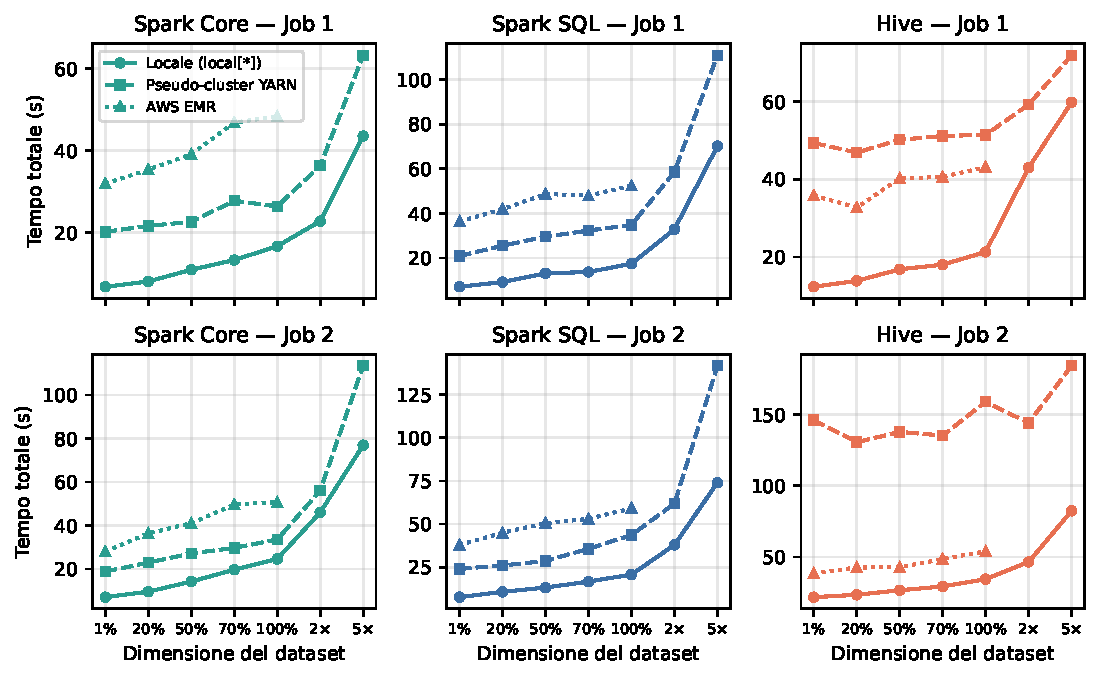
\includegraphics[width=\textwidth]{generato/fig_ambienti.pdf}
\caption{Tempo totale al variare della dimensione del dataset nei tre ambienti (su EMR dall'1\% al 100\%).}
\label{fig:ambienti}
\end{figure}

\begin{table}[H]
\centering\small
\begin{tabular}{@{}l l r r r r r@{}}
\toprule
Job & Tecnologia & Locale & YARN & AWS EMR & YARN/Locale & AWS/Locale \\
\midrule
\multirow{3}{*}{Job 1} & Spark Core & 14,6 & 29,7 & 48,3 & 2,04$\times$ & 3,32$\times$ \\
 & Spark SQL & 14,5 & 37,3 & 52,4 & 2,57$\times$ & 3,61$\times$ \\
 & Hive & 19,5 & 53,9 & 43,1 & 2,76$\times$ & 2,21$\times$ \\
\midrule
\multirow{3}{*}{Job 2} & Spark Core & 20,8 & 33,5 & 50,8 & 1,61$\times$ & 2,44$\times$ \\
 & Spark SQL & 17,1 & 39,1 & 59,1 & 2,28$\times$ & 3,45$\times$ \\
 & Hive & 30,1 & 138,6 & 54,0 & 4,61$\times$ & 1,80$\times$ \\
\bottomrule
\end{tabular}
\caption{Tempo totale (s) sul dataset completo nei tre ambienti e rapporto rispetto al locale.}
\label{tab:ambienti}
\end{table}

\begin{figure}[H]
\centering
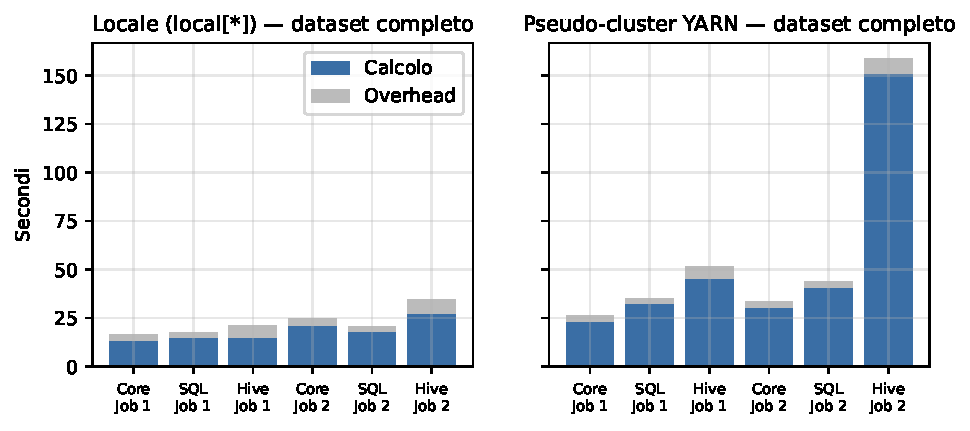
\includegraphics[width=\textwidth]{generato/fig_overhead.pdf}
\caption{Tempo di calcolo e overhead sul dataset completo in locale e su YARN.}
\label{fig:overhead}
\end{figure}

\begin{table}[H]
\centering\small
\begin{tabular}{@{}c l l l r r r@{}}
\toprule
Dataset & Job & Tecnologia & Job lanciati & Stage & Task & MB scambiati \\
\midrule
100\% & Job 1 & Spark Core & 5 job & 7 & 11 & 0,2 (shuffle) \\
100\% & Job 1 & Spark SQL & 8 job & 8 & 11 & 0,4 (shuffle) \\
100\% & Job 1 & Hive & 2 MR & -- & -- & 206 (HDFS) \\
\midrule
100\% & Job 2 & Spark Core & 5 job & 10 & 25 & 1,4 (shuffle) \\
100\% & Job 2 & Spark SQL & 14 job & 14 & 23 & 2,7 (shuffle) \\
100\% & Job 2 & Hive & 6 MR & -- & -- & 413 (HDFS) \\
\midrule
5× & Job 1 & Spark Core & 5 job & 7 & 43 & 0,6 (shuffle) \\
5× & Job 1 & Spark SQL & 8 job & 8 & 35 & 1,6 (shuffle) \\
5× & Job 1 & Hive & 2 MR & -- & -- & 1.028 (HDFS) \\
\midrule
5× & Job 2 & Spark Core & 5 job & 10 & 113 & 4,5 (shuffle) \\
5× & Job 2 & Spark SQL & 14 job & 14 & 84 & 10,9 (shuffle) \\
5× & Job 2 & Hive & 6 MR & -- & -- & 2.057 (HDFS) \\
\bottomrule
\end{tabular}
\caption{Metriche del motore su YARN: job, stage e task di Spark con i MB scritti nello shuffle; job MapReduce di Hive
con i MB letti da HDFS.}
\label{tab:metriche}
\end{table}

%==============================================================================================
\section{Analisi critica}\label{sec:critica}
%==============================================================================================
\subsection{Espressività}
Spark SQL e Hive esprimono ciascun job con una sola query dichiarativa: raggruppamenti, espressioni condizionali per
le fasce, funzioni finestra per la classifica delle cause e join esterno sono costrutti nativi, e il piano di
esecuzione è scelto dal sistema. In Spark Core la stessa logica va costruita a mano: accumulatori per le
aggregazioni, gestione esplicita dei valori mancanti, due pipeline e un join per il Job~2, ordinamento e intestazione
dell'output. Le righe di codice significative (Tabella~\ref{tab:loc}) lo riflettono solo in parte, perché gli script
SQL includono anche la definizione della tabella e le colonne di output; la differenza vera è che in Spark Core ogni
riga è logica da scrivere e verificare. Spark Core è però il più flessibile: qualunque struttura (per esempio un
insieme di mesi) può fare da accumulatore, senza dipendere dalle funzioni disponibili. Hive ha il dialetto più
limitato, e la portabilità tra versioni non è garantita: \code{array\_join} esiste in Hive 4 ma non in Hive 3.

\begin{table}[H]
\centering\small
\begin{tabular}{@{}l r r@{}}
\toprule
Tecnologia & Job 1 & Job 2 \\
\midrule
Spark Core & 79 & 105 \\
Spark SQL & 48 & 75 \\
Hive & 35 & 83 \\
\bottomrule
\end{tabular}
\caption{Righe di codice significative per job (escluse righe vuote, commenti e stampe di servizio).}
\label{tab:loc}
\end{table}

\subsection{Semplicità implementativa}
Spark SQL è stato il più semplice: la query si scrive e si verifica come in un database. Spark Core ha richiesto più
attenzione ai dettagli semantici che SQL gestisce da solo: tre dei difetti emersi dalla verifica (massimo falsato dai
voli senza ritardo, medie in arrivo con valori mancanti contati come zero, ordine delle cause a pari frequenza)
riguardavano la versione RDD o la sua coerenza con SQL. Hive, a parità di query, è il più oneroso da mettere in
esercizio: metastore, compatibilità con Java 21, intestazioni non ignorate, tipi (\code{FLOAT} contro
\code{DOUBLE}) e formato dei valori mancanti hanno richiesto interventi specifici.

\subsection{Efficienza}
\begin{itemize}
  \item \textbf{Dataset piccoli}: il tempo è dominato dai costi fissi. In locale sull'1\% Spark impiega circa
        \T{local}{spark-core}{job_1}{flights_1}--\T{local}{spark-sql}{job_2}{flights_1}\,s, di cui il
        \OVH{local}{spark-core}{job_1}{flights_1}\,\% (Spark Core, Job 1) è overhead di avvio; Hive paga l'avvio di un
        job MapReduce per ogni fase (\T{local}{hive}{job_1}{flights_1}\,s per il Job 1 e
        \T{local}{hive}{job_2}{flights_1}\,s per il Job 2, che ne lancia \M{hive_mr:job_2}).
  \item \textbf{Dataset grandi, in locale}: sul $5\times$ Spark Core è il più veloce nel Job 1
        (\T{local}{spark-core}{job_1}{flights_x5}\,s contro \T{local}{spark-sql}{job_1}{flights_x5}\,s di Spark SQL e
        \T{local}{hive}{job_1}{flights_x5}\,s di Hive), mentre nel Job 2 le tre tecnologie sono vicine
        (\T{local}{spark-core}{job_2}{flights_x5}, \T{local}{spark-sql}{job_2}{flights_x5} e
        \T{local}{hive}{job_2}{flights_x5}\,s). Il divario di Spark SQL nel Job 1 dipende dal numero di letture
        dell'input: l'event log mostra \SC{n}{spark-sql}{job_1} letture complete da 1\,GB (inferenza dello schema,
        \SC{1}{spark-sql}{job_1}\,s; anteprima con \code{show}, \SC{2}{spark-sql}{job_1}\,s; scrittura,
        \SC{3}{spark-sql}{job_1}\,s), perché ogni azione su un DataFrame non in cache riesegue la query. Spark Core
        legge l'input una sola volta: le azioni successive riusano i file di shuffle già
        prodotti e Spark salta gli stage già calcolati.
  \item \textbf{YARN}: lo stesso hardware diventa più lento (Tabella~\ref{tab:ambienti}): sul dataset completo da
        \RY{spark-core}{job_2} a \RY{spark-sql}{job_2} volte per Spark e fino a \RY{hive}{job_2} volte per il Job 2 di
        Hive. Il costo è in gran parte dentro il tempo di calcolo (Figura~\ref{fig:overhead}): richiesta dei container
        a YARN, avvio delle JVM degli executor e, per Spark, solo 2 executor da un core contro gli 8 thread del
        locale. Hive lo paga a ogni job MapReduce: il Job 2 resta tra \T{yarn}{hive}{job_2}{flights_20} e
        \T{yarn}{hive}{job_2}{flights_x5}\,s a ogni dimensione.
  \item \textbf{AWS EMR}: con questi volumi il cluster è più lento del locale (da \RA{hive}{job_2} a
        \RA{spark-sql}{job_1} volte sul dataset completo): tre nodi, rete e coordinamento non vengono ripagati da
        appena \DS{mb}{flights_cleaned}\,MB. Hive, che su EMR usa Tez (un unico grafo di esecuzione invece di job
        MapReduce separati), è il più veloce nel Job 1 (\T{aws}{hive}{job_1}{flights_cleaned}\,s contro
        \T{aws}{spark-core}{job_1}{flights_cleaned} e \T{aws}{spark-sql}{job_1}{flights_cleaned}\,s).
\end{itemize}

\subsection{Scalabilità}
Moltiplicando l'input per 100 (dall'1\% al 100\%) i tempi crescono molto meno che linearmente: in locale di
\GU{local}{hive}{job_2}--\GU{local}{spark-core}{job_2} volte, su YARN di \GU{yarn}{hive}{job_1}--\GU{yarn}{spark-core}{job_2}
volte, su EMR di \GU{aws}{hive}{job_1}--\GU{aws}{spark-core}{job_2} volte, perché fino al dataset completo prevalgono i
costi fissi. Oltre, la crescita si avvicina a quella dei dati: da 100\% a $5\times$ (input $\times 5$) in locale
Spark Core cresce di \GC{local}{spark-core}{job_1}--\GC{local}{spark-core}{job_2} volte e Spark SQL di
\GC{local}{spark-sql}{job_2}--\GC{local}{spark-sql}{job_1}, penalizzato dalle letture ripetute. Hive in locale cresce
in modo simile a Spark Core (\GC{local}{hive}{job_2}--\GC{local}{hive}{job_1} volte), mentre su YARN cresce molto meno
(\GC{yarn}{hive}{job_2}--\GC{yarn}{hive}{job_1} volte, contro \GC{yarn}{spark-core}{job_1}--\GC{yarn}{spark-core}{job_2} di
Spark Core) perché lì il suo costo fisso è molto più alto: al $5\times$ Hive supera Spark SQL nel Job 1
(\T{yarn}{hive}{job_1}{flights_x5} contro \T{yarn}{spark-sql}{job_1}{flights_x5}\,s). Le curve di Spark e Hive tendono
quindi a incrociarsi al crescere dell'input: il vantaggio dell'esecuzione in memoria è netto sui volumi piccoli e
medi e si riduce quando domina la lettura dei dati. La dimensione del cluster EMR è rimasta fissa; con questi volumi
più nodi aumenterebbero soprattutto il coordinamento.

\subsection{Shuffle, aggregazione e preparazione dei dati}
\begin{itemize}
  \item \textbf{Shuffle}: i dati scambiati sono pochi MB anche con 1\,GB di input (Tabella~\ref{tab:metriche}):
        \M{shuffle:spark-core:job_1:flights_x5}\,MB per Spark Core e \M{shuffle:spark-sql:job_2:flights_x5}\,MB per
        Spark SQL nel Job 2 sul $5\times$. Entrambi aggregano \emph{prima} dello shuffle (\code{reduceByKey} combina in
        ogni partizione, Catalyst usa un'aggregazione hash parziale), e le chiavi sono poche (circa 1.700 coppie
        compagnia-aeroporto, 4.000 aeroporto-mese). Il costo dominante è quindi leggere e interpretare il CSV, non
        scambiare dati.
  \item \textbf{Materializzazione in Hive}: ogni job MapReduce scrive il proprio risultato su HDFS e il successivo lo
        rilegge; inoltre la query del Job 2 legge l'input due volte (fasce e cause), come mostrano i
        \M{hive_read:job_2:flights_cleaned}\,MB letti per \DS{mb}{flights_cleaned}\,MB di input.
  \item \textbf{Valutazione pigra}: in Spark SQL il Job 2 legge l'input \SC{n}{spark-sql}{job_2} volte (inferenza dello
        schema, poi due rami della query, fasce e cause, sia per l'anteprima sia per la scrittura). Uno schema esplicito
        e la cache del risultato prima delle due azioni eliminerebbero la maggior parte di queste letture. In Spark Core
        la cache dell'input del Job 2 evita solo in parte la doppia lettura, perché le due pipeline sono eseguite in
        stage paralleli (\SC{1}{spark-core}{job_2} e \SC{2}{spark-core}{job_2}\,s sul $5\times$).
  \item \textbf{Preparazione}: ridurre il file da \Q{colonne_iniziali} a 9 colonne (da 1,2\,GB a
        \DS{mb}{flights_cleaned}\,MB) riduce di circa sei volte il volume letto da ogni esecuzione di ogni job, che è
        proprio la componente dominante. Anche le altre scelte hanno effetto sulle prestazioni: i codici espliciti
        permettono di contare insieme cancellazioni e ritardi con un solo \code{UNION ALL}, e i dataset come cartelle
        HDFS evitano copie preliminari.
\end{itemize}

%==============================================================================================
\section{Conclusioni}
%==============================================================================================
Le tre tecnologie producono risultati identici. Spark SQL offre il miglior rapporto tra espressività e semplicità ed è
competitivo sui volumi piccoli e medi, a patto di controllare le letture ripetute dovute alla valutazione pigra e
all'inferenza dello schema. Spark Core è il più veloce quando la pipeline è semplice, perché legge l'input una volta e
riusa i risultati intermedi, ma richiede molto più codice e attenzione ai dettagli semantici. Hive ha il costo fisso più
alto, per l'avvio dei job MapReduce e la materializzazione dei risultati intermedi, ma scala in modo più regolare al
crescere dell'input ed è competitivo su EMR con Tez. Sui volumi di questo dataset il fattore dominante è l'overhead
di avvio e coordinamento, più che la capacità di calcolo: per questo il locale batte YARN ed EMR, e la preparazione
dei dati, che riduce il volume letto, conta più delle differenze negli shuffle.

\appendix
\section{Riproducibilità}
Il repository (\url{\repo}) contiene un modulo per tecnologia (\code{spark-core/}, \code{spark-sql/}, \code{hive/},
ciascuno con \code{run.sh} per l'ambiente locale e \code{run\_aws.sh} per EMR), la preparazione dei dati
(\code{dataset/}), l'esecuzione e la misura dei job (\code{bench/}, \code{benchmark.py}), la verifica
(\code{verify\_outputs.py}), una dashboard Streamlit per lanciare i job e consultarne tempi, stage, log e risultati
(\code{dashboard/}), i risultati (\code{results/}) e i sorgenti di questa relazione. Il README descrive installazione
e configurazione; i passi essenziali sono:
\begin{lstlisting}[language=bash]
pip install -r requirements.txt && cd dataset && python3 download.py   # dataset (token Kaggle)
bash generate_data.sh "local[*]" && cd ..                             # preparazione, porzioni, repliche, HDFS
python3 benchmark.py job_1 yarn && python3 benchmark.py job_2 yarn    # anche "local[*]" o dalla dashboard
python3 verify_outputs.py job_1 && python3 verify_outputs.py job_2
python3 docs/relazione/genera_dati.py && cd docs/relazione && tectonic main.tex
\end{lstlisting}

\end{document}
